\newpage
\thispagestyle{empty}
\mbox{}

\chapter{Parrafor en sucio}
\label{ch:chapter6}


En donde, $\sigma$ es la desviación típica aportando información sobre la variación de la concentración de las sustancias y $\mu$ la media que representa el punto de máxima radiación de la fuente. Un aspecto relevante es que si el centro de la formación se encuentra lo suficientemente cerca de la fuente el argumento de la exponencial tenderá a 0 conllevando a que en torno a dicho punto se tenga la máxima concentración de sustancias.

\begin{figure}[htb]
\centering
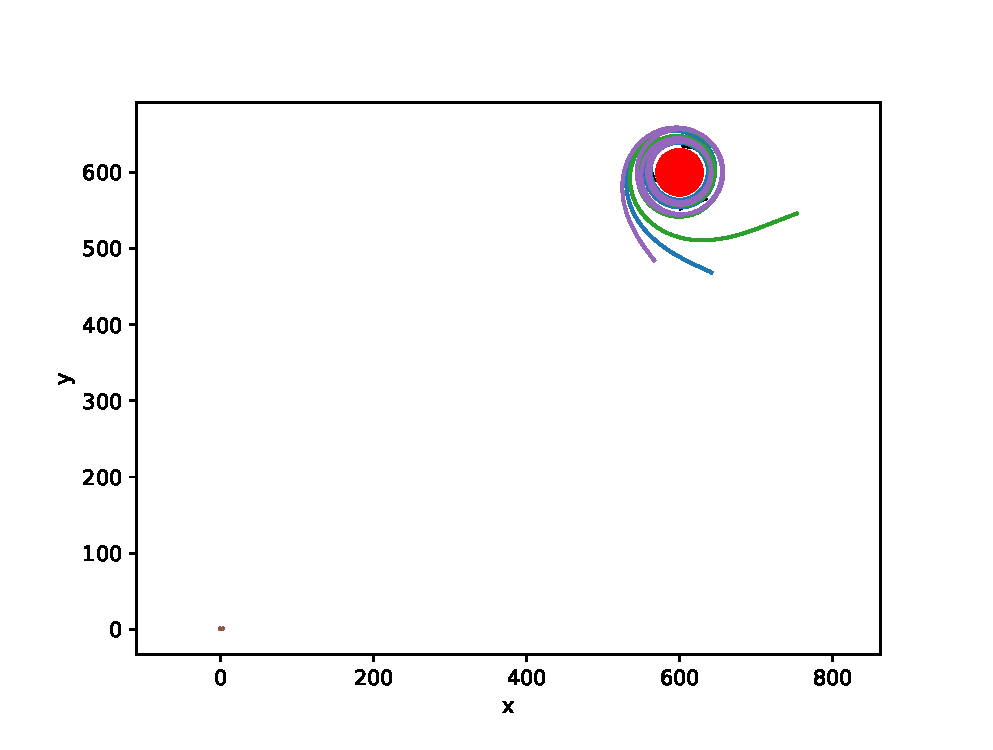
\includegraphics[width=0.85\textwidth]{figures/Coordinacion/Objetivo_Final.eps}
\caption{Vehículos dispuestos en torno a la formación. El punto rojo representa el circulo al que quieren converger y las diferentes líneas que giran en torno a dicho punto son cada una de las trayectorias de los vehículos.} \label{Ejemplo_Coordinacion}
\end{figure}

\begin{figure}[htb]
\centering
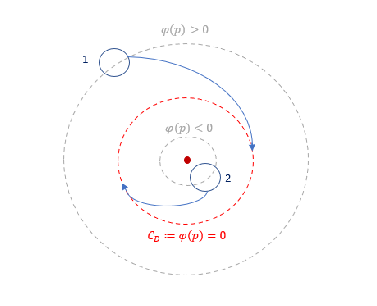
\includegraphics[width=0.60\textwidth]{figures/Pruea_Coordinacion.eps}
\caption{Ejemplo del algoritmo de control de formación} \label{Ejemplo_Coordinacion}
\end{figure}

No obstante, el algoritmo a su vez debería de estar acotado por el número de agentes que a pesar de influir en menor medida también deben de tomarse en cuenta para dicha cota.